\chapter{Funktionsscharen}

\section{Definition}
\begin{flushleft}
    Eine Funktionsschar ist eine Funktion, die auch von anderen Parametern als $x$ abhängt.
    Durch einen weiteren Parameter kann es plötzlich unendlich viele Variationen von der ursprünglichen Funktion geben.
    Das ist auch der Grund dafür, dass solch eine Funktion, Funktionsschar genannt wird.
    Es entsteht eine Menge -- also ein Schar -- von Funktionen.
\end{flushleft}

\section{Beispiel}
\begin{flushleft}
    Das ist beispielsweise eine quadratische Funktionsschar, die von den Parametern $x$ und $k$ abhängt.
    \begin{align}
        f_k(x)=kx^2
    \end{align}
    Der Parameter $k$ bestimmt nur die Stauchung der Funktion.
\end{flushleft}

\begin{center}
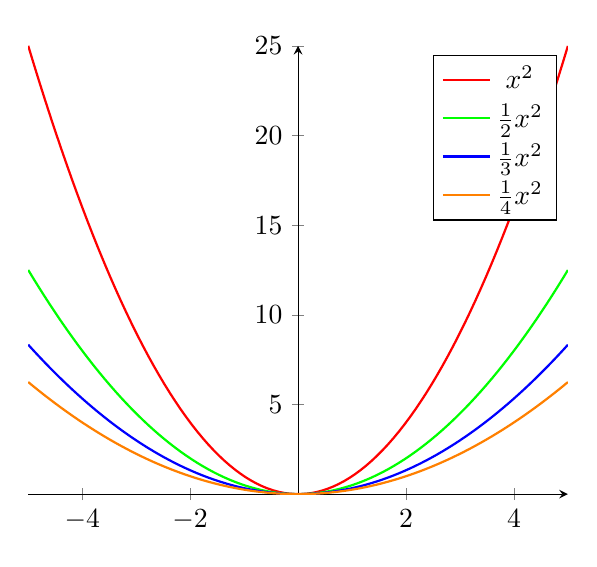
\begin{tikzpicture}
\begin{axis}[
    axis lines=middle,
    samples=100,
    domain=-5:5,
    every axis plot/.append style={thick},
]
\addplot[
    color=red,
]
{x^2};
\addlegendentry{$x^2$}

\addplot[
    color=green,
]
{0.5*x^2};
\addlegendentry{$\frac{1}{2}x^2$}

\addplot[
    color=blue,
]
{0.3333*x^2};
\addlegendentry{$\frac{1}{3}x^2$}

\addplot[
    color=orange,
]
{0.25*x^2};
\addlegendentry{$\frac{1}{4}x^2$}

\end{axis}
\end{tikzpicture}
\end{center}
